%% LyX 2.3.7 created this file.  For more info, see http://www.lyx.org/.
%% Do not edit unless you really know what you are doing.
\documentclass[12pt,hyperfootnotes=false]{article}
\usepackage[latin9]{inputenc}
\usepackage{geometry}
\geometry{verbose,tmargin=1in,bmargin=1in,lmargin=1in,rmargin=1in}
\usepackage{float}
\usepackage{amsmath}
\usepackage{amsthm}
\usepackage{amssymb}
\usepackage{graphicx}
\usepackage{setspace}
\usepackage{booktabs}

\usepackage[authoryear]{natbib}
\onehalfspacing

\makeatletter

%%%%%%%%%%%%%%%%%%%%%%%%%%%%%% LyX specific LaTeX commands.
%% Because html converters don't know tabularnewline
\providecommand{\tabularnewline}{\\}

%%%%%%%%%%%%%%%%%%%%%%%%%%%%%% User specified LaTeX commands.
\usepackage{amsthm}
\usepackage{bm}
\usepackage{setspace}
\usepackage{sectsty}

\usepackage{datetime}
\usepackage{pdflscape}
\usepackage[english]{babel}
\usepackage[small]{caption}
\usepackage[bottom,hang,flushmargin]{footmisc}

\DeclareMathOperator{\sgn}{sgn}
\DeclareMathOperator{\Var}{Var}
\DeclareMathOperator{\Corr}{Corr}
\DeclareMathOperator{\Cov}{Cov}
\DeclareMathOperator{\E}{E}
\DeclareMathOperator{\logit}{logit}
\DeclareMathOperator{\I}{I}

\sectionfont{\noindent\normalfont\large\bf}
\subsectionfont{\noindent\normalfont\normalsize\bf}
\subsubsectionfont{\noindent\normalfont\it}

\pdfminorversion=4

\makeatother

\begin{document}
\title{\noindent \textbf{Econ 220A Homework 1}}
\author{\noindent Shiqi Yang,\textbf{ }\textit{UC Berkeley}\textbf{}\thanks{E-mail:\ shiqiy@berkeley.edu
}\textbf{}\\
}
\date{\today}
\maketitle

\begin{spacing}{1.4}

\section{Question 1}

See ``Hw2/repo/analysis/code/q1\_shares\_module.py" as reference of calculating market shares.

\section{Question 2}


See ``Hw2/repo/analysis/code/q2\_invert.py" as reference of the algorithm. The values of $\delta$ are presented below. We can have $log(s_{jct}) - log(s_{0ct}) = \delta_{jct}$.

\begin{table}[htbp]
    \centering
    \caption{Delta Comparison in City 1, Period 1 (\(\sigma=0.0\))}
    \label{tab:q2_delta_city1_period1_sigma0p0}
\toprule
\begin{tabular}{rrrrrr}
\toprule
city & period & product & delta_hat & delta_log_s_minus_log_s0 & difference \\
\midrule
\midrule
1.0000 & 1.0000 & 1.0000 & -0.5791 & -0.5791 & -0.0000 \\
1.0000 & 1.0000 & 2.0000 & -0.5919 & -0.5919 & -0.0000 \\
1.0000 & 1.0000 & 3.0000 & -0.8362 & -0.8362 & -0.0000 \\
1.0000 & 1.0000 & 4.0000 & -1.0016 & -1.0016 & 0.0000 \\
1.0000 & 1.0000 & 5.0000 & -0.7629 & -0.7629 & -0.0000 \\
\bottomrule
\bottomrule
\end{tabular}

\end{table}


\section{Question 3}


Let $s(\delta,\sigma)$ denote the $J$-vector of market shares implied by the random-coefficients logit with a single random coefficient on $x_j=X_j^s-\bar X^s$. For each simulation draw $i$ with $v_i$ we define
\[
s_{ij}=\frac{\exp\{\delta_j+\sigma v_i x_j\}}{1+\sum_{m=1}^J \exp\{\delta_m+\sigma v_i x_m\}},
\qquad
s_i=(s_{i1},\ldots,s_{iJ})^\top,
\]
and approximate $s(\delta,\sigma)=\mathbb{E}_i[s_i]$ by averaging over the $N$ draws.

Observed shares satisfy the implicit system $s(\delta(\sigma),\sigma)=s^{\text{obs}}$. By the Implicit Function Theorem,
\[
\frac{\partial \delta}{\partial \sigma}
= -\left(\frac{\partial s}{\partial \delta}\right)^{-1}
\left(\frac{\partial s}{\partial \sigma}\right).
\]
For a given draw $i$,
\[
\frac{\partial s_i}{\partial \delta}
=\operatorname{diag}(s_i)-s_i s_i^{\top},
\qquad
\left(\frac{\partial s_i}{\partial \sigma}\right)_j
= v_i\, s_{ij}\big(x_j - s_i^{\top}x\big).
\]
Taking expectations over draws,
\[
\frac{\partial s}{\partial \delta}
=\mathbb{E}_i\!\left[\operatorname{diag}(s_i)-s_i s_i^{\top}\right] \equiv \mathbf{J},
\qquad
\left(\frac{\partial s}{\partial \sigma}\right)_j
=\mathbb{E}_i\!\left[v_i\, s_{ij}\big(x_j - s_i^{\top}x\big)\right] \equiv (g_\sigma)_j.
\]
Hence,
\[
\boxed{
\frac{\partial \delta(\sigma)}{\partial \sigma}
= -\,\mathbf{J}^{-1}\,g_\sigma
}
\]
with $\mathbf{J}$ and $g_\sigma$ defined above. 


\section{Question 4}

See  ``Hw2/repo/analysis/code/q4\_blp\_results.py" as reference of the algorithm.

\section{Question 5}

We construct a cost-shifter instrument following Problem Set~1:
\[
Z^{CS}_{jct} = \text{distance}_{jc} \times \text{diesel}_t,
\]
where $\text{distance}_{jc}$ is the distance between city $c$ and product $j$'s distribution center, and $\text{diesel}_t$ is the diesel price in period $t$. This variable affects prices through marginal costs but is excluded from the demand equation. The final instrument matrix is
\[
Z = [Z^{CS},\ \text{product FE},\ \text{city FE},\ \text{time FE}],
\quad W = (Z'Z)^{-1}.
\]

For a given $\sigma$ and simulated heterogeneity draws $v_i$, we compute $\delta(\sigma)$ via the Berry contraction:
\[
\delta^{(n+1)} = \delta^{(n)} + [\log s^{obs} - \log s(\delta^{(n)},\sigma)].
\]
We then estimate the linear parameters by IV:
\[
\hat{\beta} = ((X'ZWZ'X)^{-1}X'ZWZ'\delta),
\quad \hat{\xi} = \delta - X\hat{\beta}.
\]
The GMM moments and objective function are:
\[
m = \frac{1}{n}Z'\hat{\xi}, \qquad G(\sigma) = 10^6\, m'Wm.
\]

Evaluating at $\sigma = 0$ and $\sigma = 10$ gives nearly identical values:
\[
G(0) = 1.45\times10^{-24}, \qquad G(10) = 1.44\times10^{-24},
\]



\begin{table}[htbp]
    \centering
    \caption{BLP Objective With Cost Shifter (Two Sigma Values)}
    \label{tab:q5_blp_costshifter_G}
\begin{tabular}{rrr}
\toprule
sigma & G & alpha \\
\midrule
\midrule
0.0000 & 0.0000 & -2.8627 \\
10.0000 & 0.0000 & -2.8783 \\
\bottomrule
\bottomrule
\end{tabular}

\end{table}


The objective function is essentially flat in $\sigma$, implying that the dispersion parameter is weakly identified. The reason that we cannot identify $\sigma$ is we do not have enough moment conditions for GMM.


\section{Question 6}

G(0) and G(10) are reported below:

\begin{table}[htbp]
    \centering
    \caption{BLP Objective With Cost Shifter And Market-Level $z_{ct}$ (Two Sigma Values)}
    \label{tab:q6_blp_costshifter_plus_z_G}
\begin{tabular}{rrr}
\toprule
sigma & G & alpha \\
\midrule
\midrule
0.0000 & 0.0049 & -3.2375 \\
10.0000 & 0.0058 & -3.2297 \\
\bottomrule
\bottomrule
\end{tabular}

\end{table}



In Question 5, the objective function was nearly flat:
\[
G(0) \approx G(10) \approx 0,
\]
implying that for any value of $\sigma$ (or more generally, $\theta_2$), one can always find linear parameters $\hat{\beta}_0$ and $\hat{\alpha}$ such that
\[
\hat{\xi}(\theta_2)' Z W Z' \hat{\xi}(\theta_2) = 0.
\]
In other words, the instruments in $Z$ (mainly the cost shifter and fixed effects) were sufficient to orthogonalize the residuals for any $\sigma$, leaving $G(\sigma)$ flat and $\sigma$ weakly identified.

When we introduce the additional instrument
\[
z_{ct} = \sum_{j \in (c,t)} X_j^s,
\]
the matrix $Z$ now contains variation that is correlated with the nonlinear component
$\sigma v_i (X_j^s - \bar{X}^s)$.
Because this new instrument captures market-level differences in the distribution of
$X_j^s$, changes in $\sigma$ affect $\delta(\sigma)$ in directions that $Z$ can no longer
completely span. Consequently, $\hat{\xi}(\sigma)$ cannot be made perfectly orthogonal to $Z$
for all $\sigma$, and
\[
G(0) = 0.0049 \neq G(10) = 0.0058.
\]
This curvature in $G(\sigma)$ means that the moments are now informative about $\sigma$:
the additional instrument helps identify $\theta_2$ by breaking the collinearity between the
nonlinear term and the linear projection space of $X$.

\section{Question 7}

See below. $\partial G/\partial \sigma$ crosses zero when G($\sigma$) reach minimum. The shape of G($\sigma$) is symmetric, and reach global minimum at around -150 and 150, it have a local minimum point at $\sigma = 0$.

\begin{figure}[H]
    \centering % Centers the figure and caption within the text width
\includegraphics[width=0.8\textwidth]{Hw2/repo/analysis/output/q7_Gsigma.png}
\end{figure}

\begin{figure}[H]
    \centering % Centers the figure and caption within the text width
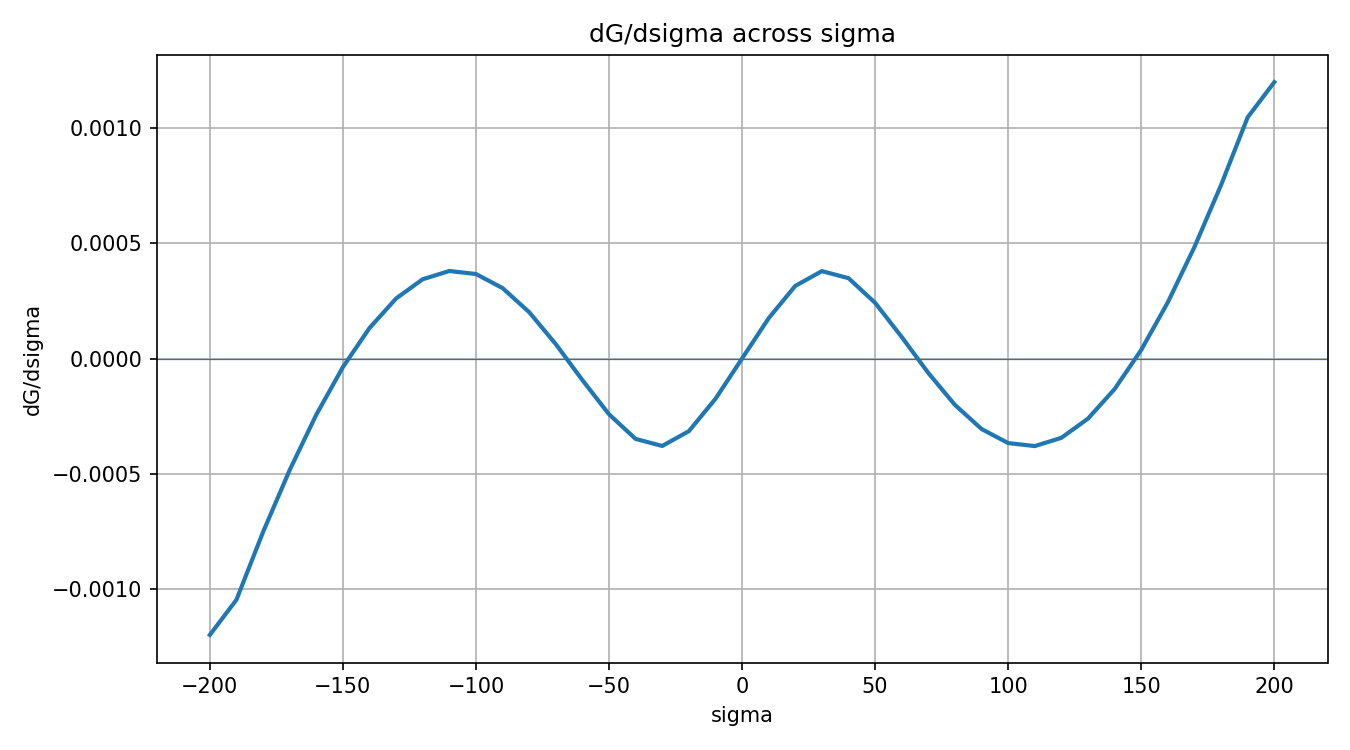
\includegraphics[width=0.8\textwidth]{Hw2/repo/analysis/output/q7_dG.png}
\end{figure}

\section{Question 8}

See below.

\begin{table}[htbp]
    \centering
    \caption{Newton Estimation Results For BLP ($\alpha$ And $\sigma$) With EHW SE}
    \label{tab:blp_q8_newton_results}
\begin{tabular}{lrr}
\toprule
parameter & estimate & se\_ehw \\
\midrule
\midrule
alpha & -4.5648 & 0.0001 \\
sigma & 148.3389 & 1.8862 \\
\bottomrule
\bottomrule
\end{tabular}

\end{table}



\section{Question 9}

See below for the cross elasticities and the diversion ratios. We can find the own elasticity did not change much. But cross-elasticities substitution patterns are larger for products with similar market share and similar sugar content. This is because random coefficient breaks IIA, so similar products have higher substitution rates.

\begin{table}[H]
    \centering
    \caption{Own- And Cross-Price Elasticities, City 1, Period 1}
    \label{tab:q9_elasticities_city1_period1}
\begin{tabular}{rrrrr}
\toprule
p@1 & p@2 & p@3 & p@4 & p@5 \\
\midrule
\midrule
-2.2465 & 0.0229 & 0.0179 & 0.7234 & 0.6127 \\
0.0161 & -2.9325 & 1.7884 & 0.0492 & 0.0170 \\
0.0161 & 2.2885 & -3.4203 & 0.0492 & 0.0170 \\
0.9702 & 0.0937 & 0.0733 & -3.4092 & 0.5058 \\
1.1891 & 0.0470 & 0.0367 & 0.7321 & -1.6767 \\
\bottomrule
\bottomrule
\end{tabular}

\end{table}


\begin{table}[htbp]
    \centering
    \caption{Diversion Ratios, City 1, Period 1}
    \label{tab:q9_diversion_city1_period1}
\toprule
\begin{tabular}{rrrrr}
\toprule
to 1 & to 2 & to 3 & to 4 & to 5 \\
\midrule
\midrule
0.0000 & 0.0071 & 0.0056 & 0.2830 & 0.4404 \\
0.0079 & 0.0000 & 0.6113 & 0.0212 & 0.0135 \\
0.0068 & 0.6675 & 0.0000 & 0.0182 & 0.0116 \\
0.3238 & 0.0217 & 0.0170 & 0.0000 & 0.2726 \\
0.4392 & 0.0121 & 0.0094 & 0.2376 & 0.0000 \\
\bottomrule
\bottomrule
\end{tabular}

\end{table}


\section{Question 10}

See below, all costs are positive.

\begin{table}[H]
    \centering
    \caption{Prices, Shares, Markups, And Marginal Costs (City 1, Period 1)}
    \label{tab:q10_results_city1_period1_single_market}
\begin{tabular}{rlrrrr}
\toprule
product & owner & price & share & markup & mc \\
\midrule
\midrule
1.0000 & prod1 & 0.7944 & 0.1658 & 0.3536 & 0.4408 \\
2.0000 & prod2 & 1.1437 & 0.1637 & 0.3900 & 0.7537 \\
3.0000 & prod3 & 1.1410 & 0.1282 & 0.3336 & 0.8074 \\
4.0000 & prod4 & 0.9037 & 0.1086 & 0.2651 & 0.6387 \\
5.0000 & prod5 & 0.4919 & 0.1379 & 0.2934 & 0.1985 \\
\bottomrule
\bottomrule
\end{tabular}

\end{table}



\section{Question 11}

See below. The prices of other products are similar to the predicts from the Logit and MNL model in PSet 1, but the BLP model predicts a higher merged prices. This is because there is not much cross elasticity to the sugar-free products, which let the firm able to set higher prices.

\begin{table}[htbp]
    \centering
    \caption{Observed vs Counterfactual Prices After Merger (City 1, Period 1)}
    \label{tab:q11_prices_counterfactual_city1_period1}
\toprule
\begin{tabular}{rrr}
\toprule
product & price_old & price_new \\
\midrule
\midrule
1.0000 & 0.7944 & 0.7932 \\
2.0000 & 1.1437 & 1.4866 \\
3.0000 & 1.1410 & 1.5404 \\
4.0000 & 0.9037 & 0.9030 \\
5.0000 & 0.4919 & 0.4909 \\
\bottomrule
\bottomrule
\end{tabular}

\end{table}


\section{Question 12}

See below. The welfare cost is -0.087, which is larger than results in Logit model -0.015 and nested logit model -0.061. This is consistent with our previous results showing that price of merged products increase more than in nest and non-nested models, which makes consumer in general worse off.

\begin{table}[htbp]
    \centering
    \caption{Consumer Surplus Before/After Merger (City 1, Period 1)}
    \label{tab:q12_welfare_city1_period1}
\toprule
\begin{tabular}{rrrrr}
\toprule
city & period & CS_no_merger & CS_merger & Delta_CS \\
\midrule
\midrule
1.0000 & 1.0000 & 0.4122 & 0.3247 & -0.0874 \\
\bottomrule
\bottomrule
\end{tabular}

\end{table}


\section{Question 13}


Problem Set #1 highlights  instruments and the choice of model are essential for identification. Problem Set #2 shows how BLP model reshape elasticities and diversion patterns, producing heterogeneous substitution across brands. Together they demonstrate that pricing, markups, and merger counterfactuals heavily depend on the model setting and the substitution pattern can be very important.

\end{spacing}
\end{document}
